\scanpage{2}
$V$ : \uline{W.d. noethérien}; Complet
\[
\operatorname{Spec}(V)\qquad k\ \text{corps \unsure{resid}}\qquad K\ \text{\unsure{corps fract\textsuperscript{s}|corps fractions}}
\]
Gpe galoisien $(K)$

a) $\operatorname{car}(\unsure{k|K})=0$\qquad \uuline{$k$ alg clos}.
\figure{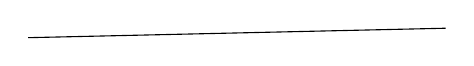
\begin{tikzpicture}\draw (0,0)--(5.3,.12);\end{tikzpicture}}
Les extens a $K$ sont \unsure{abel.} cyclique donc kummerienne.
\[
K^*/K^{*n}\simeq\mathbf Z/n\mathbf Z\qquad\text{(par la valuation)}
\]
Soit $\overline K$ clôture a $K$.
\diagram{\begin{tikzcd}[ampersand replacement=\&,column sep=small,row sep=small]
\Gamma(\overline K,K) \arrow[r,phantom,"\overset{\text{not}}{=}"] \& T_\infty(k) \arrow[r,phantom,"="] \& \displaystyle\varprojlim_n\underbrace{\mu_n(k)} \arrow[d,phantom,"\wr"] \& (\simeq\widehat{\mathbf Z})\\
\&\&\mathbf Z/n\mathbf Z
\end{tikzcd}}
\figure{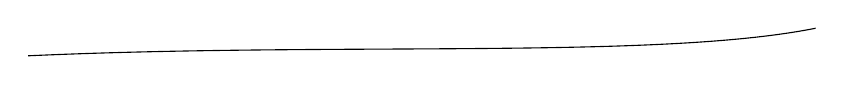
\begin{tikzpicture}\draw (0,0)..controls (4,.18) and (8,-.05)..(10,.35);\end{tikzpicture}}
si $k$ car $\unsure{\ne0}$ $V$ pas neces complet,
\[
\underset{\text{prem à }p}{\pi_1(K)}\longrightarrow\varprojlim_{n\text{ prem à }p}\mu_n(k)
\]
\mspage{1}
